% GNUPLOT: LaTeX picture with Postscript
\begingroup
  \makeatletter
  \providecommand\color[2][]{%
    \GenericError{(gnuplot) \space\space\space\@spaces}{%
      Package color not loaded in conjunction with
      terminal option `colourtext'%
    }{See the gnuplot documentation for explanation.%
    }{Either use 'blacktext' in gnuplot or load the package
      color.sty in LaTeX.}%
    \renewcommand\color[2][]{}%
  }%
  \providecommand\includegraphics[2][]{%
    \GenericError{(gnuplot) \space\space\space\@spaces}{%
      Package graphicx or graphics not loaded%
    }{See the gnuplot documentation for explanation.%
    }{The gnuplot epslatex terminal needs graphicx.sty or graphics.sty.}%
    \renewcommand\includegraphics[2][]{}%
  }%
  \providecommand\rotatebox[2]{#2}%
  \@ifundefined{ifGPcolor}{%
    \newif\ifGPcolor
    \GPcolortrue
  }{}%
  \@ifundefined{ifGPblacktext}{%
    \newif\ifGPblacktext
    \GPblacktexttrue
  }{}%
  % define a \g@addto@macro without @ in the name:
  \let\gplgaddtomacro\g@addto@macro
  % define empty templates for all commands taking text:
  \gdef\gplbacktext{}%
  \gdef\gplfronttext{}%
  \makeatother
  \ifGPblacktext
    % no textcolor at all
    \def\colorrgb#1{}%
    \def\colorgray#1{}%
  \else
    % gray or color?
    \ifGPcolor
      \def\colorrgb#1{\color[rgb]{#1}}%
      \def\colorgray#1{\color[gray]{#1}}%
      \expandafter\def\csname LTw\endcsname{\color{white}}%
      \expandafter\def\csname LTb\endcsname{\color{black}}%
      \expandafter\def\csname LTa\endcsname{\color{black}}%
      \expandafter\def\csname LT0\endcsname{\color[rgb]{1,0,0}}%
      \expandafter\def\csname LT1\endcsname{\color[rgb]{0,1,0}}%
      \expandafter\def\csname LT2\endcsname{\color[rgb]{0,0,1}}%
      \expandafter\def\csname LT3\endcsname{\color[rgb]{1,0,1}}%
      \expandafter\def\csname LT4\endcsname{\color[rgb]{0,1,1}}%
      \expandafter\def\csname LT5\endcsname{\color[rgb]{1,1,0}}%
      \expandafter\def\csname LT6\endcsname{\color[rgb]{0,0,0}}%
      \expandafter\def\csname LT7\endcsname{\color[rgb]{1,0.3,0}}%
      \expandafter\def\csname LT8\endcsname{\color[rgb]{0.5,0.5,0.5}}%
    \else
      % gray
      \def\colorrgb#1{\color{black}}%
      \def\colorgray#1{\color[gray]{#1}}%
      \expandafter\def\csname LTw\endcsname{\color{white}}%
      \expandafter\def\csname LTb\endcsname{\color{black}}%
      \expandafter\def\csname LTa\endcsname{\color{black}}%
      \expandafter\def\csname LT0\endcsname{\color{black}}%
      \expandafter\def\csname LT1\endcsname{\color{black}}%
      \expandafter\def\csname LT2\endcsname{\color{black}}%
      \expandafter\def\csname LT3\endcsname{\color{black}}%
      \expandafter\def\csname LT4\endcsname{\color{black}}%
      \expandafter\def\csname LT5\endcsname{\color{black}}%
      \expandafter\def\csname LT6\endcsname{\color{black}}%
      \expandafter\def\csname LT7\endcsname{\color{black}}%
      \expandafter\def\csname LT8\endcsname{\color{black}}%
    \fi
  \fi
    \setlength{\unitlength}{0.0500bp}%
    \ifx\gptboxheight\undefined%
      \newlength{\gptboxheight}%
      \newlength{\gptboxwidth}%
      \newsavebox{\gptboxtext}%
    \fi%
    \setlength{\fboxrule}{0.5pt}%
    \setlength{\fboxsep}{1pt}%
    \definecolor{tbcol}{rgb}{1,1,1}%
\begin{picture}(6060.00,4520.00)%
    \gplgaddtomacro\gplbacktext{%
      \csname LTb\endcsname%%
      \put(1041,2659){\makebox(0,0)[r]{\strut{}\scriptsize $10^{-13}$}}%
      \csname LTb\endcsname%%
      \put(1041,2966){\makebox(0,0)[r]{\strut{}\scriptsize $10^{-10}$}}%
      \csname LTb\endcsname%%
      \put(1041,3272){\makebox(0,0)[r]{\strut{}\scriptsize $10^{-7}$}}%
      \csname LTb\endcsname%%
      \put(1041,3579){\makebox(0,0)[r]{\strut{}\scriptsize $10^{-4}$}}%
      \csname LTb\endcsname%%
      \put(1041,3885){\makebox(0,0)[r]{\strut{}\scriptsize $10^{-1}$}}%
      \csname LTb\endcsname%%
      \put(1358,2516){\makebox(0,0){\strut{}\scriptsize $10^{2}$}}%
      \csname LTb\endcsname%%
      \put(1926,2516){\makebox(0,0){\strut{}\scriptsize $10^{4}$}}%
      \csname LTb\endcsname%%
      \put(2493,2516){\makebox(0,0){\strut{}\scriptsize $10^{6}$}}%
    }%
    \gplgaddtomacro\gplfronttext{%
      \csname LTb\endcsname%%
      \put(1789,2352){\makebox(0,0){\strut{}\scriptsize \# of frequencies}}%
      \csname LTb\endcsname%%
      \put(1789,4254){\makebox(0,0){\strut{}truncation and aliasing $L_2$-error}}%
    }%
    \gplgaddtomacro\gplbacktext{%
      \csname LTb\endcsname%%
      \put(4061,2659){\makebox(0,0)[r]{\strut{}\scriptsize $10^{0}$}}%
      \csname LTb\endcsname%%
      \put(4061,2977){\makebox(0,0)[r]{\strut{}\scriptsize $10^{2}$}}%
      \csname LTb\endcsname%%
      \put(4061,3295){\makebox(0,0)[r]{\strut{}\scriptsize $10^{4}$}}%
      \csname LTb\endcsname%%
      \put(4061,3613){\makebox(0,0)[r]{\strut{}\scriptsize $10^{6}$}}%
      \csname LTb\endcsname%%
      \put(4061,3931){\makebox(0,0)[r]{\strut{}\scriptsize $10^{8}$}}%
      \csname LTb\endcsname%%
      \put(4378,2516){\makebox(0,0){\strut{}\scriptsize $10^{2}$}}%
      \csname LTb\endcsname%%
      \put(4946,2516){\makebox(0,0){\strut{}\scriptsize $10^{4}$}}%
      \csname LTb\endcsname%%
      \put(5513,2516){\makebox(0,0){\strut{}\scriptsize $10^{6}$}}%
    }%
    \gplgaddtomacro\gplfronttext{%
      \csname LTb\endcsname%%
      \put(4809,2352){\makebox(0,0){\strut{}\scriptsize \# of frequencies}}%
      \csname LTb\endcsname%%
      \put(4809,4254){\makebox(0,0){\strut{}\# of points}}%
    }%
    \gplgaddtomacro\gplbacktext{%
      \csname LTb\endcsname%%
      \put(1040,409){\makebox(0,0)[r]{\strut{}\scriptsize $10^{-8}$}}%
      \csname LTb\endcsname%%
      \put(1040,727){\makebox(0,0)[r]{\strut{}\scriptsize $10^{-6}$}}%
      \csname LTb\endcsname%%
      \put(1040,1045){\makebox(0,0)[r]{\strut{}\scriptsize $10^{-4}$}}%
      \csname LTb\endcsname%%
      \put(1040,1363){\makebox(0,0)[r]{\strut{}\scriptsize $10^{-2}$}}%
      \csname LTb\endcsname%%
      \put(1040,1681){\makebox(0,0)[r]{\strut{}\scriptsize $10^{0}$}}%
      \csname LTb\endcsname%%
      \put(1252,266){\makebox(0,0){\strut{}\scriptsize $10^{2}$}}%
      \csname LTb\endcsname%%
      \put(1608,266){\makebox(0,0){\strut{}\scriptsize $10^{4}$}}%
      \csname LTb\endcsname%%
      \put(1964,266){\makebox(0,0){\strut{}\scriptsize $10^{6}$}}%
      \csname LTb\endcsname%%
      \put(2320,266){\makebox(0,0){\strut{}\scriptsize $10^{8}$}}%
    }%
    \gplgaddtomacro\gplfronttext{%
      \csname LTb\endcsname%%
      \put(1789,102){\makebox(0,0){\strut{}\scriptsize \# of points}}%
      \csname LTb\endcsname%%
      \put(1789,2004){\makebox(0,0){\strut{}$L_2$-error}}%
    }%
    \gplgaddtomacro\gplbacktext{%
      \csname LTb\endcsname%%
      \put(4060,409){\makebox(0,0)[r]{\strut{}\scriptsize $10^{-4}$}}%
      \csname LTb\endcsname%%
      \put(4060,727){\makebox(0,0)[r]{\strut{}\scriptsize $10^{-2}$}}%
      \csname LTb\endcsname%%
      \put(4060,1045){\makebox(0,0)[r]{\strut{}\scriptsize $10^{0}$}}%
      \csname LTb\endcsname%%
      \put(4060,1363){\makebox(0,0)[r]{\strut{}\scriptsize $10^{2}$}}%
      \csname LTb\endcsname%%
      \put(4060,1681){\makebox(0,0)[r]{\strut{}\scriptsize $10^{4}$}}%
      \csname LTb\endcsname%%
      \put(4378,266){\makebox(0,0){\strut{}\scriptsize $10^{2}$}}%
      \csname LTb\endcsname%%
      \put(4946,266){\makebox(0,0){\strut{}\scriptsize $10^{4}$}}%
      \csname LTb\endcsname%%
      \put(5513,266){\makebox(0,0){\strut{}\scriptsize $10^{6}$}}%
    }%
    \gplgaddtomacro\gplfronttext{%
      \csname LTb\endcsname%%
      \put(4809,102){\makebox(0,0){\strut{}\scriptsize \# of frequencies}}%
      \csname LTb\endcsname%%
      \put(4809,2004){\makebox(0,0){\strut{}time in seconds}}%
    }%
    \gplbacktext
    \put(0,0){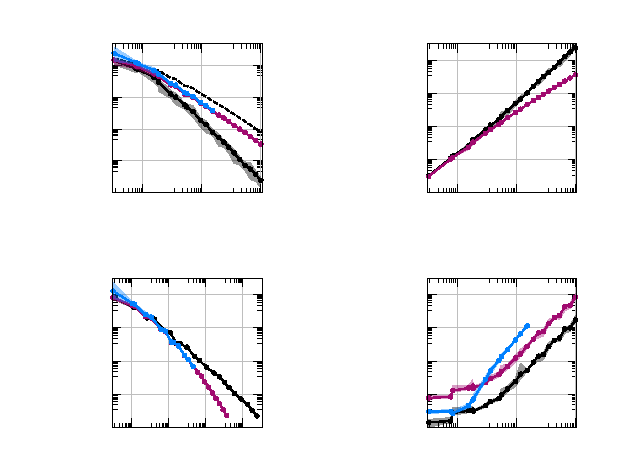
\includegraphics[width={303.00bp},height={226.00bp}]{img/wc_rand}}%
    \gplfronttext
  \end{picture}%
\endgroup
